\question 某信道传输速率为4kbit/s,采用停止-等待协议。传播时延t=20ms,确认帧长度和处理时间均可忽略,帧长达到(
)才能使信道的利用率达到至少50\%
\par\twoch{40bit}{80bit}{\textcolor{red}{160bit}}{320bit}
\begin{solution}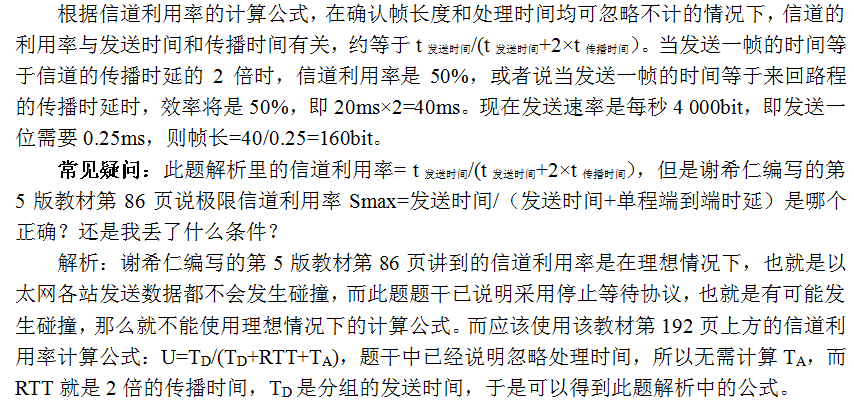
\includegraphics[width=3.70833in,height=1.76042in]{computerassets/4852416235FE9EA14F68B05403BF782C.png}
\end{solution}
\question 与CSMA/CD网络相比较,令牌环网更适合的环境是
\par\twoch{负载轻}{\textcolor{red}{负载重}}{距离远}{距离近}
\begin{solution}CSMA/CD协议在网络负载较重时会因为碰撞而造成效率的降低,而令牌环网络因为使用了令牌环来避免网络中的冲突,与CSMA/CD协议相比,减少了冲突率,提高了网络传输速率。
\end{solution}
\question (华中科技大学,2001年)长度为10km,数据传输率为10Mbit/s的CSMA/CD以太网,信号传播速度为200m/us,那么该网络的最小帧长为
\par\twoch{20bit}{200bit}{100bit}{\textcolor{red}{1000bit}}
\begin{solution}概念题
\end{solution}
\question CSMA/CD以太网中,发生冲突后,重发前的退避时间最大是
\par\twoch{65536个时间片}{65535个时间片}{1024个时间片}{\textcolor{red}{1023个时间片}}
\begin{solution}设重发前的退避时间为r个时间片,由退避算法的定义知r={[}0,1,
,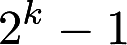
\includegraphics[width=0.45833in,height=0.16667in]{texmath/2116a45Cdpi7B3507D25Ek-1}{]}中的一个随机数,因为k=min{[}重传次数,10{]},易知k不大于10,故r不大于1023。
\end{solution}
\question CSMA协议可以利用多种监听算法来减小发送冲突的概率,下列关于各种监听算法的描述中,正确的是
\par\fourch{非坚持型监听算法有利于减少网络空闲时间}{1-坚持型监听算法有利于减小冲突的概率}{P-坚持型监听算法无法减少网络的空闲时间}{\textcolor{red}{1-坚持型监听算法能够及时抢占信道}}
\begin{solution}按总线争用协议来分类,CSMA有3种类型:
1)非坚持CSMA。一个站点在发送数据帧前,先要对媒介进行检测。如果没有其他站点在发送数据,那么该站点开始发送数据。如果媒介被占用,那么该站点不会持续监听媒介,而等待一个随机的延迟时间之后再监听。采用随机的监听延迟时间可以减少发生冲突的可能性,但其缺点也是很明显的:即使有多个站点有数据要发送,因为此时所有站点可能都在等待各自的随机延迟时间,而媒介仍然可能处于空闲状态,所以就使得媒介的利用率较低,故排除选项A。
2)1-坚持CSMA。当一个站点要发送数据帧时,它就监听媒介,判断当前时刻是否有其他站点正在传输数据。如果媒介忙的话,该站点等待直至媒介空闲。一旦该站点检测到媒介空闲,它就立即发送数据帧,故D选项是正确的。如果产生冲突,则等待一个随机时间再监听。之所以叫``1-坚持'',是因为当一个站点发现媒介空闲时,它传输数据帧的概率为1。1-坚持CSMA的优点:只要媒介空闲,站点就立即发送,它的缺点:假如有两个或两个以上的站点有数据要发送,冲突就不可避免,排除选项B。
3)P-坚持CSMA。P-坚持CSMA是非坚持CSMA和1-坚持CSMA的折中。P-坚持CSMA应用于划分时槽的媒介,其工作过程如下:当一个站点要发送数据帧时,它先检测媒介。若媒介空闲,则该站点按照概率P的可能性发送数据,同时有1-P的概率会把要发送数据帧的任务延迟到下一个时槽。按照这样的规则,若下一个时槽也是空闲的,则站点同样按照概率P的可能性发送数据,如果处理得当,P-坚持型监听算法还是可以减少网络的空闲时间的,故排除选项C。
\end{solution}
\question 全双工以太网传输技术的特点是( )。 Ⅰ.能同时发送和接收帧
Ⅱ.不受CSMA/CD限制 Ⅲ.不能同时发送和接收帧 Ⅳ.受CSMA/CD限制
\par\twoch{\textcolor{red}{Ⅰ,Ⅱ}}{Ⅰ,Ⅳ}{Ⅱ,Ⅲ}{Ⅲ,Ⅳ}
\begin{solution}因为全双工既有接收数据的通道又有发送数据的通道,所以能同时发送和接收帧。CSMA/CD协议是防止发送和接收冲突的协议,而全双工根本不存在冲突,所以不受CSMA/CD的限制。
\end{solution}
\question 在二进制后退算法中,如果发生了12次碰撞,那么站点会在0~(
)之间选择一个随机数
\par\twoch{\textcolor{red}{1023}}{1024}{4095}{4096}
\begin{solution}概念题
\end{solution}
\question 以太网中如果发生介质访问冲突,按照二进制指数后退算法决定下一次重发的时间,使用二进制后退算法的理由是
\par\twoch{这种算法简单}{这种算法执行速度快}{\textcolor{red}{这种算法考虑了网络负载对冲突的影响}}{这种算法与网络的规模大小无关}
\begin{solution}以太网采用CSMA/CD技术,当网络上的流量越多,负载越大时,发生冲突的几率也会越大。当工作站发送的数据帧因冲突而传输失败时,会采用二进制后退算法后退一段时间后重新发送数据帧。二进制后退算法可以动态地适应发送站点的数量,后退延时的取值范围与重发次数n形成二进制指数关系。当网络负载小时,后退延时的取值范围也小;而当负载大时,后退延时的取值范围也随着增大。二进制后退算法的优点是把后退延时的平均取值与负载的大小联系起来。所以,二进制后退算法考虑了网络负载对冲突的影响。
\end{solution}
\question 在以太网上``阻塞''信号的功能是
\par\fourch{当发现冲突时,CSMA/CA发送一个“阻塞”信号。当所有的站都检测到阻塞信号时,它们立即停止发送尝试}{\textcolor{red}{当发现冲突时,CSMA/CD发送一个“阻塞”信号。当所有的站都检测到阻塞信号时,它们立即停止发送尝试}}{当发现冲突时,CSMA/CD发送一个“阻塞”信号。当所有的站都检测到阻塞信号时,它们立即开始竞争访问介质}{当发现冲突时,CSMA/CA发送一个“阻塞”信号。当所有的站都检测到阻塞信号时,它们立即开始竞争访问介质}
\begin{solution}属于理解性的题目,见知识点讲解
\end{solution}
\question 在一个采用CSMA/CD协议的网络中,传输介质是一根完整的电缆,传输速率为1Gbit/s,电缆中的信号传播速度是200
000km/s。若最小数据帧长度减少800比特,则最远的两个站点之间的距离至少需要(
)
\par\twoch{增加160m}{增加80m}{减少160m}{\textcolor{red}{减少80m}}
\begin{solution}知识点复习:
1)若最短帧长减少,而数据传输速率不变,则需要将冲突域的最大距离缩短来保证争用期的减少。从该描述中可以得出,此题答案一定是减少站点之间的距离,可以先排除A和B选项。
2)争用期:指网络中源主机和目标主机之间的往返时延,如果经过争用期这段时间还没有检测到冲突,才能肯定这次发送不会发生冲突。因此,争用期也指数据没有发生冲突的最长时间。
争用期=(2×s)/信号的传播速度
争用期还有一种表述方式,即直接使用比特作为单位:
争用期=数据帧长度/数据帧传输速率
有了以上争用期的两个表达式,只需列出一个一元一次方程即可解决这一类问题。
最小数据帧长减少800bit,假设最远的两个站点之间距离需要减少s米,则可以得到下面的一元一次方程:
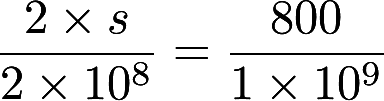
\includegraphics[width=1.37500in,height=0.36458in]{texmath/5dab885Cdpi7B3507D5Cfrac7B25Ctimes7Bs7D7D7B25Ctimes105E87D3D5Cfrac7B8007D7B15Ctimes105E97D}解得:s=80m。
\end{solution}
